\documentclass[12pt]{report}

\usepackage[spanish]{babel}
\usepackage[none]{hyphenat}
\usepackage[left=1.5cm, right=1.5cm, top = 2cm, bottom=2.5cm]{geometry}
\usepackage{parskip}
\usepackage[export]{adjustbox}
\usepackage{enumitem}[shortlabels]
\usepackage{graphicx}
\usepackage{caption} 
\usepackage{wrapfig}
\usepackage{xcolor}
\usepackage{longtable}
\usepackage{multirow, makecell}
\usepackage{amsmath} 
\usepackage{amsfonts}
\usepackage[hidelinks]{hyperref}
\usepackage{csquotes}
\usepackage{helvet}
\usepackage{pgfplots}

\newcommand{\linejump}{\hfill \break}
\renewcommand{\familydefault}{\sfdefault}

\definecolor{azuloscuro}{RGB}{0,0,128}

\sloppy
\decimalpoint
\graphicspath{{img/}}

\begin{document}
  \noindent
  \begin{center}
    \textbf{UNIVERSIDAD NACIONAL AUTÓNOMA DE MÉXICO \\
    FACULTAD DE INGENIERÍA \\
    DIVISIÓN DE CIENCIAS BÁSICAS \\
    COORDINACIÓN DE CIENCIAS APLICADAS \\
    SEGUNDO EXAMEN PARCIAL DE PROBABILIDAD}
  \end{center}

  \linejump

  \textbf{Profesora} Act. Nora Patricia Rocha Miller \hfill \textbf{15 de noviembre de 2023} \\
  \textbf{Semestre 2024-1} \hfill \textbf{FECHA DE ENTREGA: 16/11/23, 23:00 horas}

  \linejump

  \textbf{Nombre:} \underline{\hspace*{2.8cm} Acosta \hspace*{2.8cm} Porcayo \hspace*{2.8cm} Alan Omar \hspace*{2.8cm}}  \\
  \hspace*{3.7cm} \textbf{Apellido paterno} \hspace*{0.75cm} \textbf{Apellido materno} \hspace*{1.8cm} \textbf{Nombre(s)}

  \linejump

  {\color{azuloscuro} Instrucciones: Lea cuidadosamente el examen antes de resolverlo. Identifique el experimento aleatorio, la variable aleatoria muestre el desarrollo completo de los que se pide utilizando la notación matemática correspondiente.}

  \linejump
  \linejump

  \begin{enumerate}
    \item Muchos productos se fabrican en masa en líneas de ensamble automatizadas. La distribución de probabilidad del tiempo entre dos llegadas sucesivas de componentes fabricadas a la salida de la línea de ensamble tiene la siguiente función de densidad

    \[
      f(x) = \left\{
      \begin{array}{ll}
          \dfrac{e^{-.05x}}{20}, & \hspace*{1cm} x > 0 \\
          0 & \hspace*{1cm} \text{en otro caso}
      \end{array}
      \right.
    \]

  \linejump
  \begin{enumerate}[label=\alph*.]
    \item ¿Qué mide la variable aleatoria $X$?

    $X$ mide el tiempo entre la salida sucesiva de dos componentes.

    \newpage
    \item Grafique la función de densidad
    
    \begin{center}
      \begin{tikzpicture}
          \begin{axis}[
            axis lines=middle,
            xlabel=$x$,
            ylabel=$f(x)$,
            xmin=0,
            ymin=0,
            grid,
          ]
          
          \addplot[
            domain=0:10,
            samples=100,
            color=blue,
            thick,
          ]
          {exp(-0.05*x)/20};
        \end{axis}
      \end{tikzpicture}
    \end{center}
    
    \item ¿Qué probabilidad hay de que un tiempo entre llegadas (el tiempo entre llegadas de dos tubos de magnetrón) sea menor de 10 segundos?
    
    \begin{align*}
      P(X < 10) &= \int_0^{10} f(x)dx = \int_0^{10} \frac{e^{-0.05x}}{20} dx = \frac{1}{20} \int_0^{10} e^{-0.05x} dx = \frac{1}{20} \left[ \frac{e^{-0.05x}}{-0.05} \right]_0^{10} \\
      &= \left[ -e^{-0.05x} \right]_0^{10} = -e^{-0.05(10)} - (-e^{-0.05(0)}) = -e^{-0.5} - (-e^0) \\
      &= -e^{-0.5} + 1 = 1 - 0.6065 = {\color{blue}\boxed{0.3935}}
    \end{align*}

    \item ¿Qué probabilidad hay de que los siguientes cuatro tiempos entre llegadas sean todos menores de 10 segundos?
    
    \begin{align*}
      P(X_1 < 10 \cap X_2 < 10 \cap X_3 < 10 \cap X_4 < 10) &= P(X_1 < 10) \cdot P(X_2 < 10) \cdot P(X_3 < 10) \\
      & \cdot P(X_4 < 10) = P(X < 10)^4 \\ 
      &= 0.3935^4 \approx {\color{blue}\boxed{0.0240}}
    \end{align*}
    
    \item Encuentre la Función de Distribución Acumulada y grafíquela
    
    \begin{align*}
      F(x) &= \int_{-\infty}^x f(t)dt = \int_{-\infty}^0 0dt + \int_0^x \frac{e^{-0.05t}}{20} dt = \frac{1}{20} \int_0^x e^{-0.05t} dt = \frac{1}{20} \left[ \frac{e^{-0.05t}}{-0.05} \right]_0^x \\ 
      &= \left[ -e^{-0.5t} \right]_0^x = -e^{-0.05x} - (-e^0) = -e^{-0.05x} + 1 = {\color{blue}\boxed{1 - e^{-0.05x}}}
    \end{align*}

    \[
      F(x) = \left\{
      \begin{array}{ll}
          1 - e^{-0.05x}, & \hspace*{1cm} x > 0 \\
          0 & \hspace*{1cm} \text{en otro caso}
      \end{array}
      \right.
    \]

    \begin{center}
      \begin{tikzpicture}
          \begin{axis}[
            axis lines=middle,
            xlabel=$x$,
            ylabel=$f(x)$,
            xmin=0,
            ymin=0,
            grid,
          ]
          
          \addplot[
            domain=0:200,
            samples=100,
            color=blue,
            thick,
          ]
          {1- exp(-0.05*x)};
        \end{axis}
      \end{tikzpicture}
    \end{center}

    \item Utilice la FDA del inciso anterior y calcule las siguientes probabilidades
    
    \begin{enumerate}[label=\alph*)]
      \item Que el tiempo entre llegadas exceda el minuto
      
      \begin{align*}
        P(X > 60) &= P(60 < X < \infty) = F(\infty) - F(60) = 1 - F(60) \\
        &= 1 - (1 - e^{-0.05(60)}) = e^{-3} \approx {\color{blue}\boxed{0.0498}}
      \end{align*}

      \item Si ya excedió 10 segundos, exceda 20 segundos
      
      \begin{align*}
        P(X > 20 \mid X > 10) &= P(20 < X < \infty \mid 10 < X < \infty) \\ 
        &= \frac{P(20 < X < \infty \cap 10 < X < \infty)}{P(10 < X < \infty)} \\
        &= \frac{P(20 < X < \infty) \cdot P(10 < X < \infty)}{P(10 < X < \infty)} \\
        &= P(20 < X < \infty) = F(\infty) - F(20) = 1 - F(20) \\
        &= 1 - (1 - e^{-0.05(20)}) = e^{-1} \approx {\color{blue}\boxed{0.3679}}
      \end{align*}
    \end{enumerate}

    \item Calcule el tiempo medio entre dos llegadas sucesivas

    \begin{align*}
      E[X] &= \int_{-\infty}^{\infty} xf(x)dx = \int_{-\infty}^0 0dx + \int_0^{\infty} \frac{xe^{-0.05x}}{20} dx = \frac{1}{20} \int_0^{\infty} xe^{-0.05x} dx 
    \end{align*}

    \begin{align*}
      u = x \hspace*{3cm} & dv = e^{-0.05x} dx \\
      du = dx \hspace*{3cm} & v = \frac{e^{-0.05x}}{-0.05} 
    \end{align*}

    \begin{align*}
      E[X] &= \frac{1}{20} \left[ \frac{xe^{-0.05x}}{-0.05} \right]_0^{\infty} - \frac{1}{20} \int_0^{\infty} \frac{e^{-0.05x}}{-0.05} dx = \left[ -xe^{-0.05x} \right]_0^\infty + \int_0^\infty e^{-0.05x} dx \\ 
      &= \left[ -xe^{-0.05x} \right]_0^\infty + \left[ \frac{e^{-0.05x}}{-0.05} \right]_0^\infty = \left[ -\infty e^{-\infty} - (-0e^0) \right] + \left[ \frac{e^{-\infty}}{-0.05} - \frac{e^0}{-0.05} \right] \\
      &= \left[ 0 + 0 \right] + \left[ 0 - \frac{1}{-0.05} \right] = \frac{1}{0.05} = {\color{blue}\boxed{20}}
    \end{align*}

    \item Calcule la varianza de $X$
    
    \begin{align*}
      \sigma^2 &= E\left[ \left( X - E[X] \right)^2 \right] = E[X^2] - E[X]^2 = \int_{-\infty}^{\infty} x^2 f(x)dx - E[X]^2 \\
      &= \int_{-\infty}^0 0dx + \int_0^{\infty} \frac{x^2e^{-0.05x}}{20} dx - 20^2 = \frac{1}{20} \int_0^{\infty} x^2e^{-0.05x} dx - 400
    \end{align*}

    \begin{align*}
      u = x^2 \hspace*{3cm} & dv = e^{-0.05x} dx \\
      du = 2xdx \hspace*{3cm} & v = \frac{e^{-0.05x}}{-0.05}
    \end{align*}

    \begin{align*}
      \sigma^2 &= \frac{1}{20} \left[ \frac{x^2e^{-0.05x}}{-0.05} \right]_0^{\infty} - \frac{1}{20} \int_0^{\infty} \frac{2xe^{-0.05x}}{-0.05} dx - 400 \\
      &= \left[ -x^2e^{-0.05x} \right]_0^\infty + 2\int_0^\infty xe^{-0.05x} dx - 400 \\
      &= \left[ -\infty e^{-\infty} - (-0e^0) \right] + 2\left[ 20(E[X]) \right] - 400 \\
      &= \left[ 0 + 0 \right] + 2\left[ 20(20) \right] - 400 = 800 - 400 = {\color{blue}\boxed{400}}
    \end{align*}

  \end{enumerate}

  \linejump
  \item La gerencia de un banco debe decidir si instalará o no un sistema de apoyo a decisiones para prestamos comerciales (un sistema de información gerencial en línea) que ayude a sus analistas a tomar este tipo de decisiones, La experiencia anterior indica que $X$, el número adicional (por año) de decisiones de préstamos correctas — aceptar buenas solicitudes de préstamos y rechazar las que tarde o temprano no podrán pagarse — atribuible al sistema de apoyo de decisiones, y $Y$ la duración (en años) de este sistema, tienen la distribución de probabilidad conjunta que se muestra en la tabla.
  \end{enumerate}

  \newpage
  \begin{figure}[h!]
    \centering
    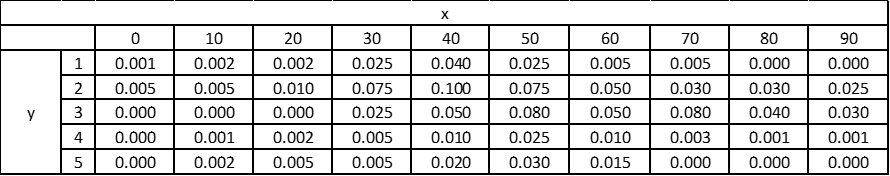
\includegraphics[width=0.9\linewidth]{T1.png}
  \end{figure}

  \linejump
  \begin{enumerate}
    \item Calcule las distribuciones de probabilidad marginal $p_X(x)$ y $p_Y(y)$
    
    \begin{align*}
      p_X(x) = \sum_y p_{XY}(x, y) = \sum_1^5 p_{XY}(x,y)
    \end{align*}

    \begin{figure}[h!]
      \centering
      
\includegraphics[width=0.9\linewidth]{Tpx.png}
    \end{figure}

    \begin{align*}
      p_Y(y) = \sum_x p_{XY}(x, y) = \sum_0^{90} p_{XY}(x,y)
    \end{align*}

    \begin{figure}[h!]
      \centering
      
\includegraphics[width=0.55\linewidth]{Tpy.png}
    \end{figure}

    \item Obtenga la distribución de probabilidad condicional $p_{X \mid Y}(x \mid y)$
    
    \begin{align*}
      p_{X \mid Y}(x \mid y) = \dfrac{p_{XY}(x, y)}{p_Y(y)}
    \end{align*}
    
    \begin{figure}[h!]
      \centering
      
\includegraphics[width=0.9\linewidth]{Tpxmy.png} 
    \end{figure}

    \newpage
    \item Dado que el sistema de apoyo a decisiones está en su tercer año de operación, calcule la probabilidad de que se tomarán por lo menos 40 decisiones de préstamos correctas adicionales.
    
    \begin{align*}
      P(X \geq 40 \mid Y = 3) &= \frac{P(X \geq 40, Y = 3)}{P(Y = 3)} \\
      &= \frac{p_{XY}(40, 3) + p_{XY}(50, 3) + p_{XY}(60, 3) + p_{XY}(70, 3) + p_{XY}(80, 3) + p_{XY}(90, 3)}{p_Y(3)} \\
      &= \frac{0.050 + 0.080 + 0.050 + 0.080 + 0.040 + 0.030}{0.355} = \frac{0.330}{0.355} \approx {\color{blue}\boxed{0.9296}}
    \end{align*}

    \item Calcule la duración esperada del sistema de apoyo a decisiones, es decir, calcule $E[Y]$
    
    \begin{align*}
      E[Y] &= \sum_y yp_Y(y) = \sum_1^5 yp_Y(y) = 1(0.105) + 2(0.405) + 3(0.355) + 4(0.058) + 5(0.077) \\
      &= 0.105 + 0.810 + 1.065 + 0.232 + 0.385 = {\color{blue}\boxed{2.597}}
    \end{align*}

    \item ¿Hay correlación entre $X$ y $Y$? ¿Son $X$ y $Y$. independientes?
    
    \textbf{Correlación:}
    
    $$\rho_{XY} = \frac{\sigma_{XY}}{\sigma_X \sigma_Y}$$
    $$\sigma_X^2 = E\left[ X^2 \right] - E[X]^2$$
    $$\sigma_Y^2 = E\left[ Y^2 \right] - E[Y]^2$$
    $$\sigma_{XY} = E\left[ XY \right] - E[X]E[Y]$$

    \begin{align*}
      E[X] &= \sum_x xp_X(x) = \sum_0^{90} xp_X(x) \\
      &= 0(0.006) + 10(0.010) + 20(0.019) + 30(0.135) + 40(0.220) + 50(0.235) \\
      &\hspace*{0.5cm} + 60(0.130) + 70(0.118) + 80(0.071) + 90(0.056) \\
      &= 0.00 + 0.10 + 0.38 + 4.05 + 8.80 + 11.75 + 7.80 + 8.26 + 5.68 + 5.04 \\
      &= 51.86
    \end{align*}

    \begin{align*}
      E\left[ X^2 \right] &= \sum_x x^2p_X(x) = \sum_0^{90} x^2p_X(x) \\
      &= 0^2(0.006) + 10^2(0.010) + 20^2(0.019) + 30^2(0.135) + 40^2(0.220) + 50^2(0.235) \\
      &\hspace*{0.5cm} + 60^2(0.130) + 70^2(0.118) + 80^2(0.071) + 90^2(0.056) \\
      &= 0.0 + 1.0 + 7.6 + 121.5 + 352.0 + 587.5 + 468.0 + 578.2 \\
      &\hspace*{0.5cm}+ 454.4 + 453.6 \\
      &= 3023.8
    \end{align*}

    \begin{align*}
      \sigma_X &= \sqrt{E\left[ X^2 \right] - E[X]^2} = \sqrt{3023.8 - 51.86^2} = \sqrt{3023.80 - 2689.46} = \sqrt{334.34} \approx 18.285 
    \end{align*}

    \begin{align*}
      E[Y] = \sum_y yp_Y(y) = \sum_1^5 yp_Y(y) = 2.597
    \end{align*}

    \begin{align*}
      E\left[ Y^2 \right] &= \sum_y y^2p_Y(y) = \sum_1^5 y^2p_Y(y) \\
      &= 1^2(0.105) + 2^2(0.405) + 3^2(0.355) + 4^2(0.058) + 5^2(0.077) \\
      &= 0.105 + 1.620 + 3.195 + 0.928 + 1.925 \\
      &= 7.773
    \end{align*}

    \begin{align*}
      \sigma_Y &= \sqrt{E\left[ Y^2 \right] - E[Y]^2} = \sqrt{7.773 - 2.597^2} = \sqrt{7.773 - 6.744} = \sqrt{1.029} \approx 1.014
    \end{align*}

    \begin{align*}
      E[XY] &= \sum_x \sum_y xy p_{XY}(x, y) = \sum_0^{90} \sum_1^5 xy p_{XY}(x, y) \\
      &= 0\left[ 1(0.001) + 2(0.005) + 3(0.000) + 4(0.000) + 5(0.000) \right] \\
      &\hspace*{0.5cm}+ 10\left[ 1(0.002) + 2(0.005) + 3(0.000) + 4(0.001) + 5(0.002) \right] \\
      &\hspace*{0.5cm}+ 20\left[ 1(0.002) + 2(0.010) + 3(0.000) + 4(0.002) + 5(0.005) \right] \\
      &\hspace*{0.5cm}+ 30\left[ 1(0.025) + 2(0.075) + 3(0.025) + 4(0.005) + 5(0.005) \right] \\
      &\hspace*{0.5cm}+ 40\left[ 1(0.040) + 2(0.100) + 3(0.050) + 4(0.010) + 5(0.020) \right] \\
      &\hspace*{0.5cm}+ 50\left[ 1(0.025) + 2(0.075) + 3(0.080) + 4(0.025) + 5(0.030) \right] \\
      &\hspace*{0.5cm}+ 60\left[ 1(0.005) + 2(0.050) + 3(0.050) + 4(0.010) + 5(0.015) \right] \\
      &\hspace*{0.5cm}+ 70\left[ 1(0.005) + 2(0.030) + 3(0.080) + 4(0.003) + 5(0.000) \right] \\
      &\hspace*{0.5cm}+ 80\left[ 1(0.000) + 2(0.030) + 3(0.040) + 4(0.001) + 5(0.000) \right] \\
      &\hspace*{0.5cm}+ 90\left[ 1(0.000) + 2(0.025) + 3(0.030) + 4(0.001) + 5(0.000) \right] \\
      &= 0.00 + 0.26 + 1.10 + 8.85 + 21.20 + 33.25 + 22.20 + 22.19 + 14.72 + 12.96 \\
      &= 136.73
    \end{align*}

    \begin{align*}
      \sigma_{XY} &= E[XY] - E[X]E[Y] = 136.73 - (51.86)(2.597) = 136.73 - 134.68 = 2.05
    \end{align*}

    \begin{align*}
      \rho_{XY} &= \frac{\sigma_{XY}}{\sigma_X \sigma_Y} = \frac{2.05}{(18.285)(1.014)} = \frac{2.05}{18.541} \approx {\color{blue}\boxed{0.111}}
    \end{align*}

    Al ser $\rho_{XY} \neq 0$, se puede concluir que {\color{blue}hay correlación} entre $X$ y $Y$.

    \linejump
    \textbf{Independencia:}

    Dada por: $p_{XY}(x, y) = p_X(x) \cdot p_Y(y)$
    
    \begin{align*}
      &\text{Con } X = 60 \text{ y } Y = 3 \\
      &p_{XY}(60, 3) = 0.050 \\
      &p_X(60) \cdot p_Y(3) = 0.130 \cdot 0.355 = 0.046 \\
      &\Rightarrow p_{XY}(60, 3) \neq p_X(60) \cdot p_Y(3)
    \end{align*}

    \begin{align*}
      &\text{Con } X = 30 \text{ y } Y = 5 \\
      &p_{XY}(30, 5) = 0.005 \\
      &p_X(30) \cdot p_Y(5) = 0.135 \cdot 0.077 = 0.010 \\
      &\Rightarrow p_{XY}(30, 5) \neq p_X(30) \cdot p_Y(5)
    \end{align*}

    \begin{align*}
      &\text{Con } X = 90 \text{ y } Y = 1 \\
      &p_{XY}(90, 1) = 0.000 \\
      &p_X(90) \cdot p_Y(1) = 0.056 \cdot 0.105 = 0.006 \\
      &\Rightarrow p_{XY}(90, 1) \neq p_X(90) \cdot p_Y(1)
    \end{align*}

    Como se puede observar, hay valores de $X$ y $Y$ que no cumplen con la condición de independencia, por lo que se puede concluir que $X$ y $Y$ {\color{blue}no son independientes.} \\

    \item Cada decisión de préstamo correcta aporta aproximadamente 25,000 dólares a las utilidades del banco: calcule la media y la desviación estándar de las utilidades adicionales atribuibles al sistema de apoyo a decisiones. (Sugerencia: utilice la distribución marginal $p_X(x)$)
    
    \textbf{Media:}
    \begin{align*}
      \mu = E[25,000X] &= 25,000E[X] = 25,000(51.86) = \$1,296,500
    \end{align*}

    \linejump
    \textbf{Desviación estándar:}
    \begin{align*}
      \sigma = \sqrt{25,000^2 \sigma_X^2} &= 25,000\sqrt{\sigma_X^2} = 25,000(18.285) = \$457,125
    \end{align*}
  \end{enumerate}
\end{document}